\chapter{Glacial Ice Segmentation of the HKH Region With Physics-Informed Data Augmentation}
\section{The Importance of Glacial Ice Segmentation}
Glacial ice segmentation refers to the problem of gathering hyperspectral images taken by satellites of different glaciers and segmenting or delineating which areas are glacial ice, which areas are debris covered ice (ice mixed with rocks), and which areas are just rocks. This problem is important in the field of geology as monitoring the amount and location of ice from glaciers such as the ones in the Hindu Kush Himalayas (HKH) is critical as these glaciers provide a source of freshwater to a big population of the world.

\section{Image Semantic Segmentation: Grouping Similar Pixels Together}
The task of semantic segmentation refers to grouping similar or related pixels of an image together, like those of a specific object. For example, grouping all the pixels of people, roads, buildings, or trees as seen in the figure below:

% https://towardsai.net/p/l/machine-learning-7
\begin{figure}[H] \centering
    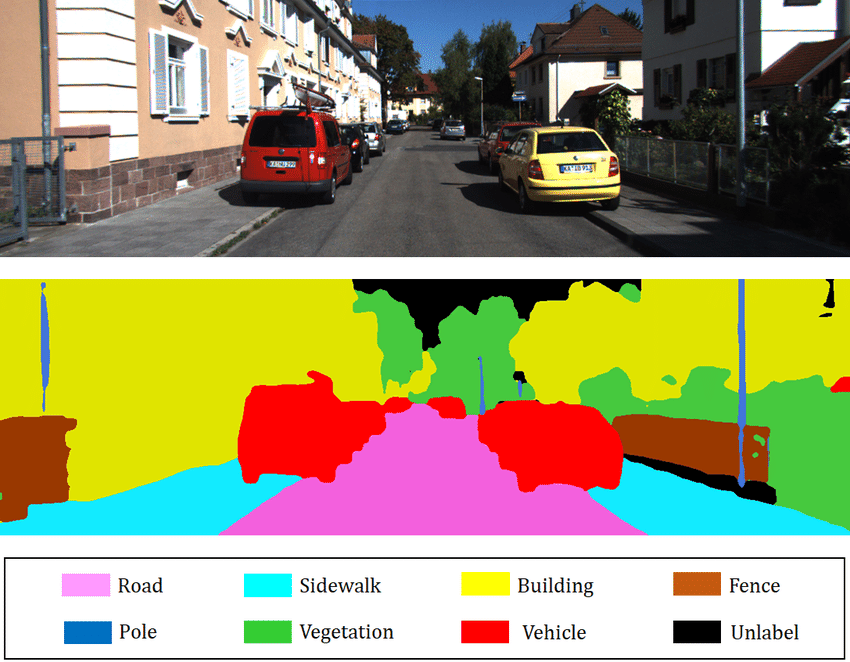
\includegraphics[width=\linewidth]{figures/semantic_segmentation.png}
    \caption{An example of semantic segmentation of an image. The pixels are grouped together by different categories.}
    \label{fig:example_semantic_segmentation}
\end{figure}

\section{Glacier Mapping Through Segmentation of Ice in Hyperspectral Images}
Glacial ice segmentation or glacier mapping is simply the task of semantic segmentation applied to hyperspectral satellite images of glaciers. The goal is to determine for each pixel in the image whether the pixel is an area of glacial ice, debris covered ice, or background (regular rocks) as shown in the figure below:

\begin{figure}[H] \centering
    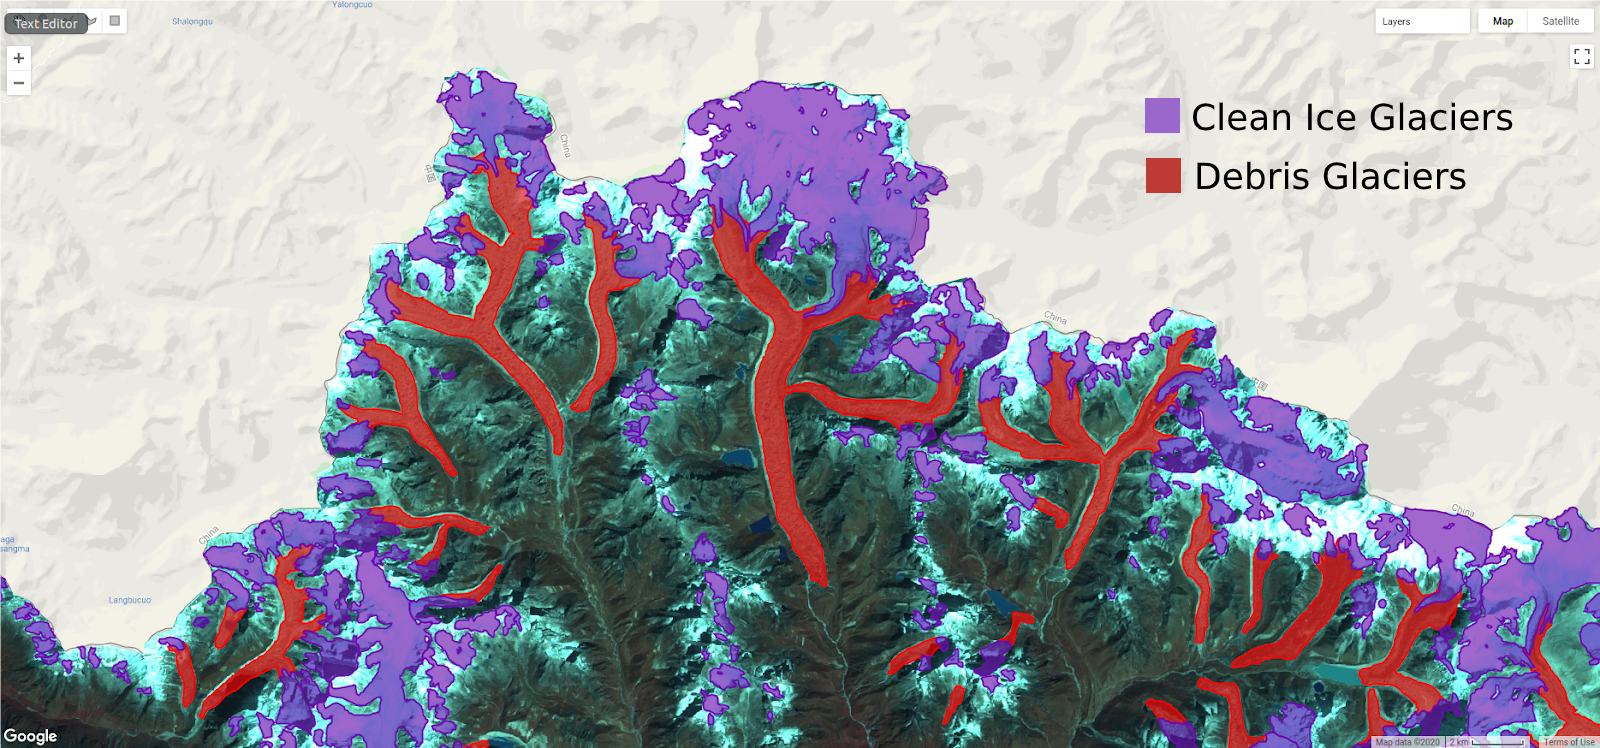
\includegraphics[width=\linewidth]{figures/glacier_mapping.png}
    \caption{Semantic segmentation of a glacier satellite image by a human annotator.}
\end{figure}


\section{Convolutional Neural Networks: The Backbone of Almost All Networks That Use Images}
Convolutional Neural Networks \cite{CNN1} are one of the most important and fundamental neural network models when dealing with datasets that contain images and their role in state-of-the-art architectures in image classification competitions such as ImageNet and other image tasks cannot be understated. CNNs operate by assuming the inputs are images and performing operations on the pixels of these images called convolutions. The purpose of these convolution operations is to apply a `filter` to extract important features out of these images as feature maps, and because these CNNs are neural networks these `filters` or `kernels` automatically learn to filter out information which might be useful for the specific task we are trying to solve. After the convolution operations a pooling operation is applied to the extracted feature maps which reduces size of these maps and the computational complexity of the network. A common pooling operation is `2x2 max-pooling` where the image is split into 2x2 patches and the maximum value at each of these patches is used to create the new reduced size feature map, the idea being that the most prominent features or those with high values are the most important for solving image problems. After extracting important features of images through convolutions and pooling layers the next step in CNNs is to convert the 2D feature maps into 1D vectors by flattening them out and then feeding these feature vectors as inputs to a regular dense network to get a final output. The layers of this dense network are typically called `fully-connected layers` to differentiate them from the `convolutional layers`.

% https://www.linkedin.com/pulse/what-convolutional-neural-network-cnn-deep-learning-nafiz-shahriar/
\begin{figure}[H] \centering
    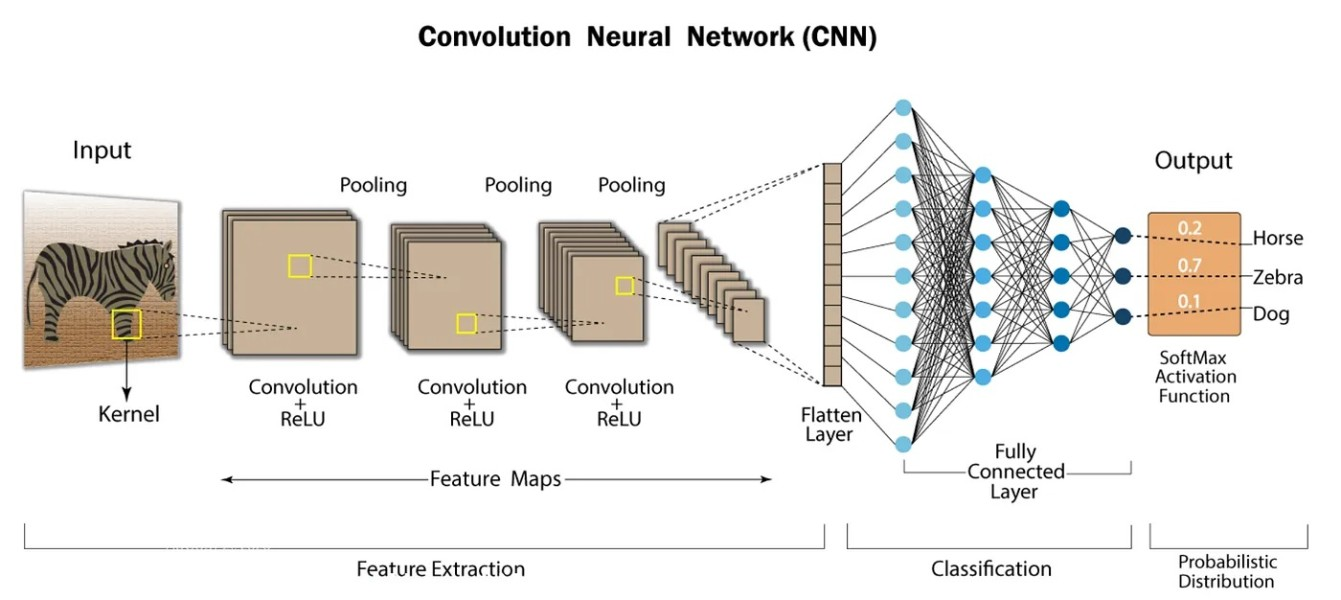
\includegraphics[width=\linewidth]{figures/cnn_architecture.jpeg}
    \caption{An example of a CNN model for an animal classification problem. Features are extracted with convolutions and pooling, and then used in a fully connected network for a final classification.}
    \label{fig:cnn_architecture}
\end{figure}


\section{UNet: The Standard Network For Image Segmentation}
U-Net \cite{UNet} is a variation of a CNN and was derived from the improvements achieved by Fully Connected Convolutional Networks (FCNs) for semantic segmentation \cite{FCN}. FCNs transform the fully-connected layers of a CNN into convolutional layers and through an upsampling strategy called `deconvolution` or `transposed convolution` output an image that is the same size as the original image. U-Net is split into two components, and encoder in the left half of the U-shape and a decoder in the right half. 

\begin{figure}[H] \centering
    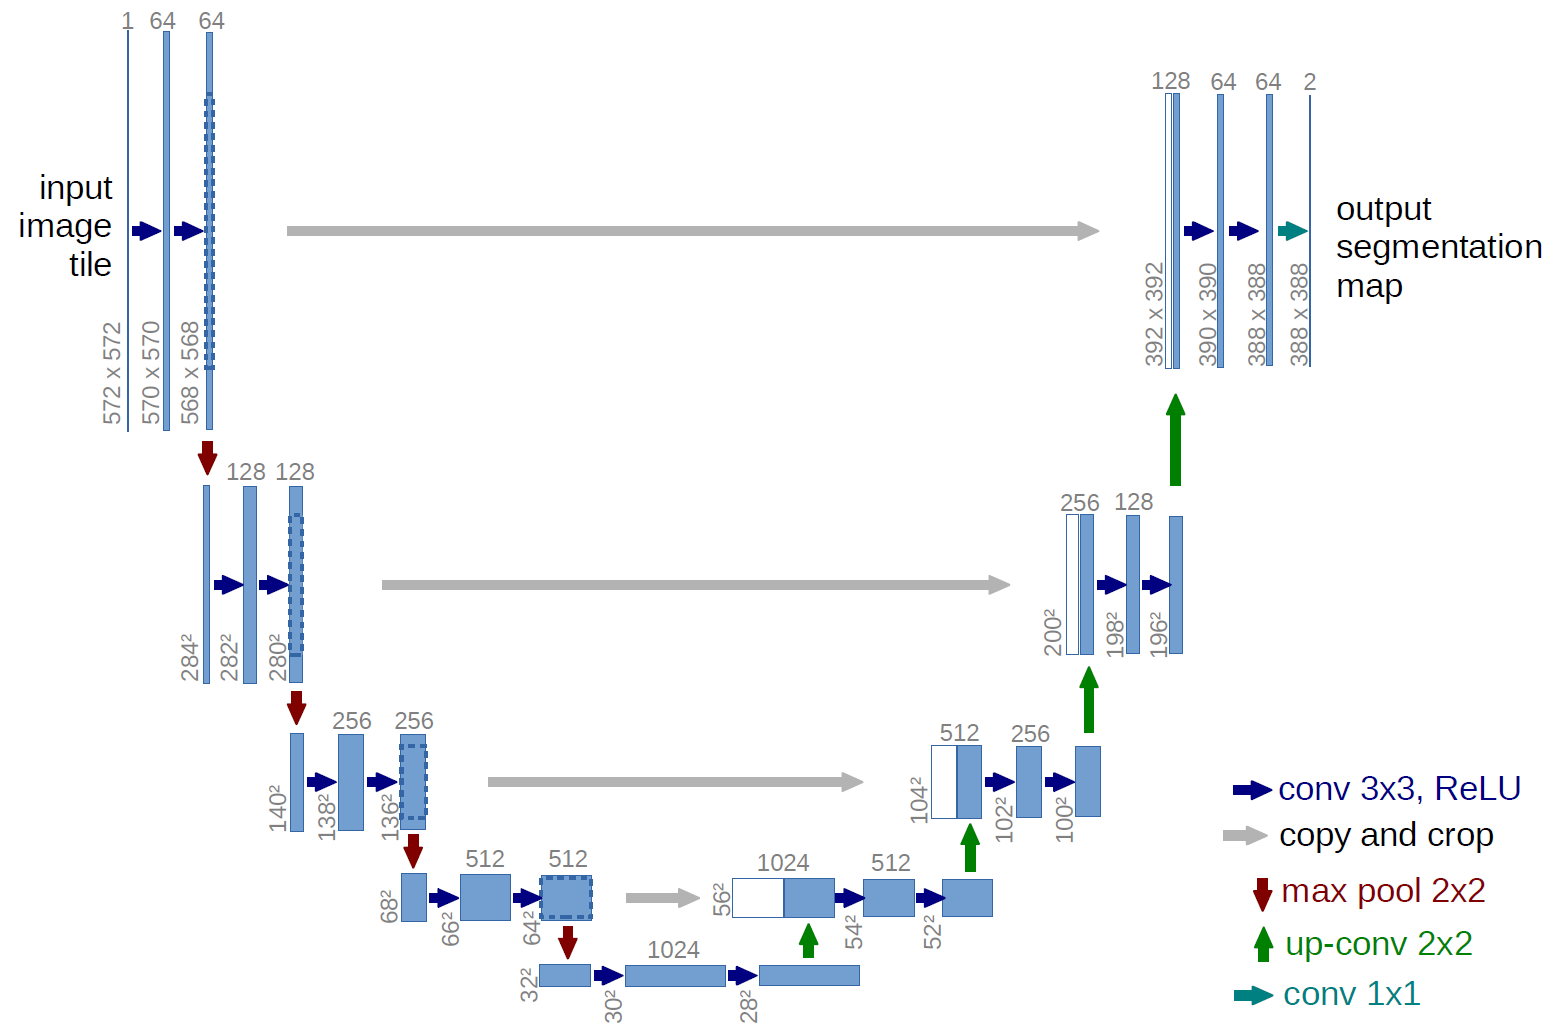
\includegraphics[width=\linewidth]{figures/unet_architecture.png}
    \caption{U-Net architecture showing both components and how they are connected to output a final segmentation map. Note the straight connections feeding previous inputs into later outputs going straight across.}
\end{figure}

The encoder also known as the contracting path is the left half of the U-shape that takes the original input image, applies regular convolutions and max-pooling, and outputs a reduced size feature map at the bottom. This is the feature extraction component that aims to capture the important context of the image.

The decoder also known as the expanding path is the right half of the U-shape that takes the feature map from the encoder and through `transposed convolutions` or `up-convolutions` upsamples and expands the feature map all the way until we get an output segmentation map which is the same size as the original input image.

Lastly, to help the decoder maintain some of the location information that is lost while encoding there are `skip-connections` going from the encoder to the decoder straight across the U-shape.

U-Net achieved state-of-the-art results when introduced in 2015 for biomedical image segmentation and these types of networks are still used to this day for many segmentation problems as a starting baseline.

\subsection{Measuring Network Performance With IoU}
% **INTRODUCING METRICS (PRECISION, RECALL, AND IOU)**
To measure the performance of the segmentation model, the main metric we used was the \textbf{Intersection over Union (IoU)} which is defined in Figure \ref{fig:iou} below and has numbers in the range from 0 to 1 with 1 being a perfect score.

\begin{figure}[H] \centering
    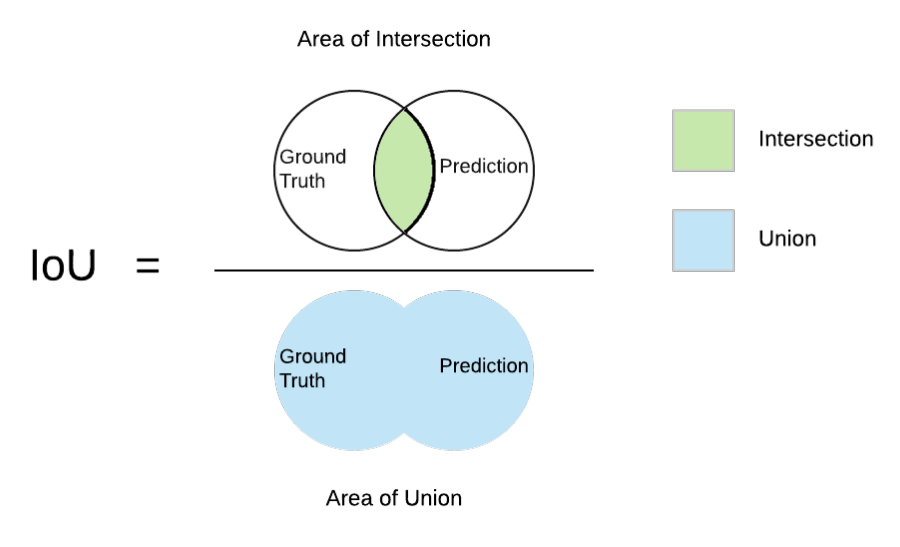
\includegraphics[width=\linewidth]{figures/iou1.png}
    \caption{Definition of Intersection over Union.}
    \label{fig:iou}
\end{figure}

\begin{figure}[H] \centering
    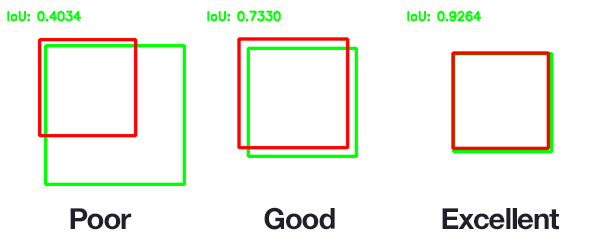
\includegraphics[width=\linewidth]{figures/iou2.png}
    \caption{Three examples of different IoU values and what type of performance they represent.}
\end{figure}

\section{Adding Physics To Image Segmentation Through Data Augmentation}
As a first step towards tackling the problem of glacial ice segmentation I began by taking a previously proposed architecture for segmentation of the Hindu Kush Himalayas (HKH) region glaciers \cite{Bibek2023} and improving its performance by adding physics to the model through data augmentation. 

The main idea was to take the elevation map from the satellite images and encode an abstract representation of a ``precipitation model'' from that elevation map as a new channel of the image. Although the actual physics equations of ice flow were not explicitly encoded in this new data channel, this new data was created from an abstract representation of the physics and we therefore called it a physics-informed data augmentation. In this channel we simulated precipitation and encoded paths where water or ice might flow from the top to the valley of the glaciers.

\begin{figure}[H] \centering
    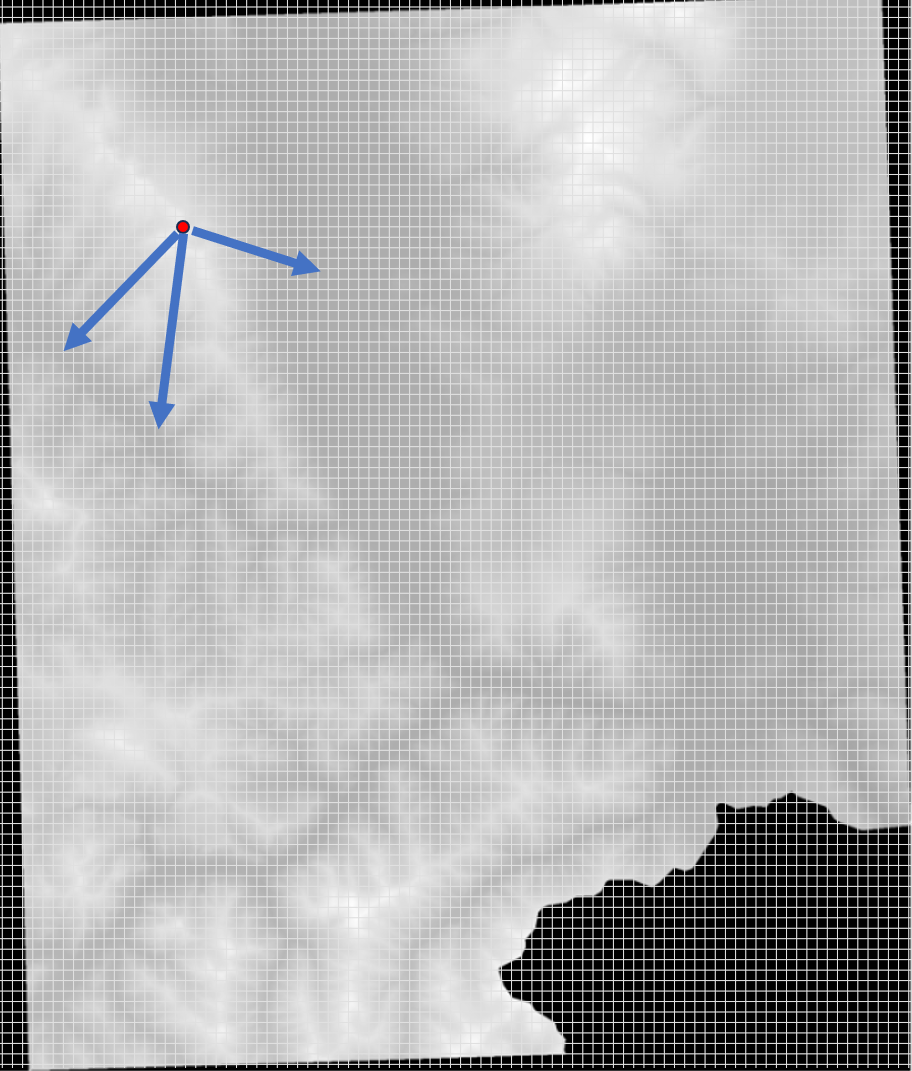
\includegraphics[width=\linewidth]{figures/data_augmentation_bfs.png}
    \caption{For each pixel in the image we simulated precipitation going down the glacier and accumulating, then we encoded such information as an additional physics-informed channel.}
    \label{fig:data_augmentation_bfs}
\end{figure}

Specifically, the algorithm as follows:
\begin{enumerate}
    \item Take the elevation map as the input image $elevation$
    \item Create an empty image of the same size as the input called $output$
    \item For each pixel in the image, perform Breadth-First Search (BFS) with a special limitation where you can only visit pixels you haven't visited before AND that are lower elevation than the current pixel popped from the queue as water/ice can only flow down.
    \item Each time a pixel is visited, the $output$ at that pixel's position increases by 1 as 1 drop of water/ice has flowed down to it.
    \item At the end, normalize the image between 0 and 1 by subtracting the mean and dividing by the standard deviation.
\end{enumerate}

In pseudocode, the data augmentation algorithm would look like:
\begin{algorithm}[H]
    \caption{Physics-Informed Data Augmentation Algorithm}
    \begin{algorithmic}
        \State $im \gets$ elevation map from satellite image
        \State $output \gets $ image full of zeros the same size as $im$
        \State $im.shape[0] \gets$ number of rows in $im$
        \State $im.shape[1] \gets$ number of columns in $im$
        \For{$u:=0 \to im.shape[0]$}
            \For{$v:=0 \to im.shape[1]$}
                \State Breadth\_First\_Search(im, output, u, v)
            \EndFor
        \EndFor
        \State $im = (im - im.mean()) / im.std()$
    \end{algorithmic}
\end{algorithm}

With the modified BFS algorithm being:
\begin{algorithm}[H]
    \caption{Physics-Informed Breadth-First Search}
    \begin{algorithmic}
        \State $im \gets$ elevation map from satellite image
        \State $output \gets$ previous accumulated output from other pixels
        \State $u \gets$ row of source pixel
        \State $v \gets$ column of source pixel
        \State $source \gets (u, v)$

        \State $visited = {source}$
        \State $Q = $ Queue with $source$ appended to it

        \While{$Q \neq Empty$}
            \State $x = Q.pop()$
            \State $curr\_elevation \gets im[x]$

            \If{$x \neq source$}
                \State $output[x] += 1$
            \EndIf

            \For{$n$ in $get\_neighbors(im, x)$}
                \State $n\_elevation \gets im[n]$
                \If{$n$ not visited $\And n\_elevation < curr\_elevation$}
                    \State Add $n$ to $visited$
                    \State Append $n$ to $Q$
                \EndIf
            \EndFor
        \EndWhile
    \end{algorithmic}
\end{algorithm}

The following figure presents an example of the results after performing the augmentation.
\begin{figure}[H] \centering
    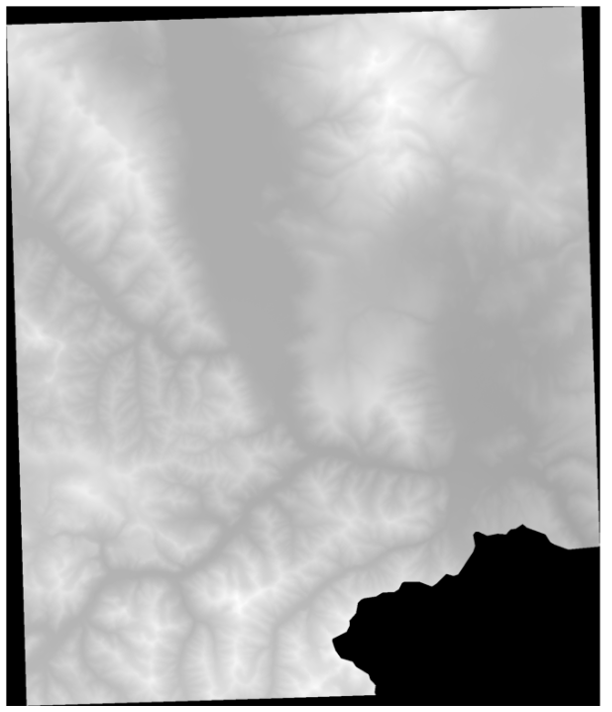
\includegraphics[width=0.45\linewidth]{figures/data_augmentation_dem.png}
    \rulesep
    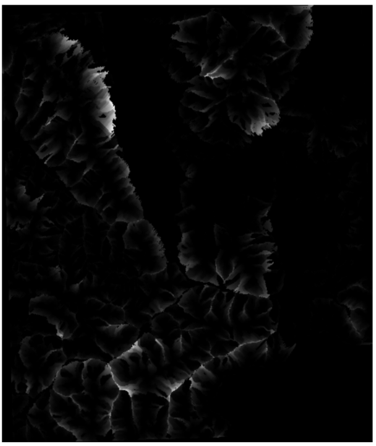
\includegraphics[width=0.45\linewidth]{figures/data_augmentation_result.png}
    \caption{Left is the elevation map from one of the glacier satellite images where white pixels are peaks and darker pixels are valleys. Right is the resulting physics-informed data augmentation channel.}
    \label{fig:data_augmentation_result}
\end{figure}


\subsection{Glacier Mapping Data From ICIMOD And Landsat7 Satellite}
The data used to train and evaluate the models were gathered and labelled by experts at the International Centre for Integrated Mountain Development (ICIMOD) from multispectral imagery from NASA's Landsat 7 satellite for the glaciers of the Hindu Kush Himalayas region from 2002 to 2008. 

\subsection{Baseline Network}
The baseline model used to evaluate our proposed data augmentation technique was the Boundary-Aware U-Net for Glacier Segmentation model developed and published in 2023 by Bibek et. al \cite{Bibek2023}. No modifications to the model were made apart from slight changes to the hyperparameter configuration and the addition of the physics-informed data augmentation technique.

\subsection{Experimental Results}
% TODO: EXPERIMENTS STILL RUNNING

% TODO: ADD IMAGE RESULTS

\begin{table}[h!]
    \centering
    \begin{tabular}{c|c|c|c}
        Model & Background IoU & CleanIce IoU & DebrisIce IoU \\ \hline
        Regular U-Net & N/A & N/A & 0.2850 \\ \hline
        Regular U-Net & N/A & 0.6560 & N/A \\ \hline
        Boundary-Aware U-Net (Baseline) & N/A & N/A & 0.3594 \\ \hline
        Boundary-Aware U-Net (Baseline) & N/A & \textbf{0.6817} & N/A \\ \hline
        \textbf{Physics \& Boundary-Aware U-Net (mine)} & 0.8640 & 0.6350 & \textbf{0.3850} \\ \hline
        
    \end{tabular}
    \caption{Comparison of the performance of different neural network models by the Intersection Over the Union (IoU) between the predicted labels and the true labels for each class. IoU is a metric between 0 and 1, with 1 being a perfect score.}
    \label{tab:my_label}
\end{table}

\subsection{Conclusion}
The current experimental results demonstrate that my proposed physics-informed data augmentation leads to improved performance for the segmentation of Debris-covered Ice from the baseline model. This is significant as classification of Debris-covered Ice is a more challenging task than that of Clean Ice for both the baseline model and expert glaciologists. With some hyper-parameter tuning I hypothesize that we can reach up to 0.40 IoU, and by switching U-Net to a newer state-of-the-art segmentation model such as MANet \cite{MANet} along with using newer loss functions such as the Unified Focal Loss \cite{UnifiedLoss} I believe we might be able to reach above 0.50 IoU. Although my proposed approach does not outperform the baseline for Clean Ice segmentation, I believe this is due to the fact that the original baseline uses two separate binary models for segmentation of each class instead of one unified multi-class model. I will train two separate binary models for a more fair comparison in the final version of my full dissertation.